\documentclass{article}
\usepackage[margin=1in]{geometry}
\usepackage{siunitx}
\usepackage{array}
\usepackage{booktabs}
\usepackage{hyperref}
\usepackage{graphicx}

\begin{document}
\author{Sachith Dunatunga}
\title{16.930 PS3}
\maketitle

\section{Convergence Study}
We have plotted the results of the convergence study in \ref{fig:cc}.
The rates are shown in table \ref{tbl:cc}.
Despite using a small time step ($\Delta t = 0.001$), we didn't quite see the expected convergence rates.
I suspect the temporal error is starting to limit the slope at larger grid sizes, as $p=2$ displays the correct behavior, but the slopes for $p = 3,4$ are a bit under what they should be.
Unfortunately, my residual evaluation code is quite slow and the largest cases already took more than an hour to run.
Switching to the given implementation did not seem to help much either with the speed, and I ran out of patience after multiple attempts.

\begin{figure}[!ht]
\centering
\begin{tabular}{c c}
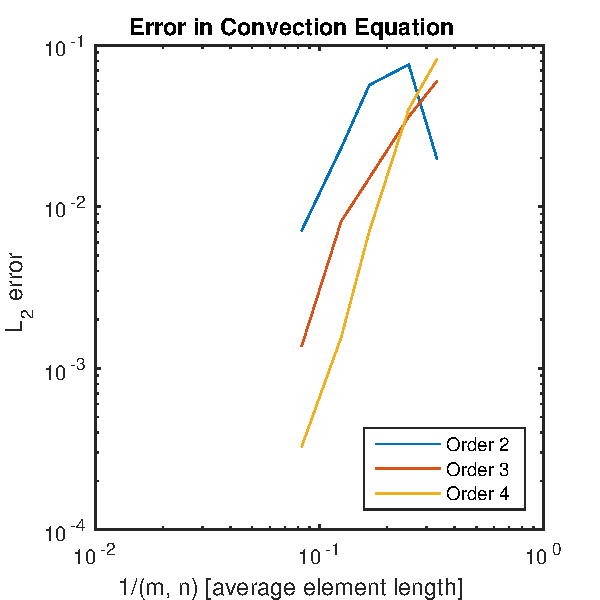
\includegraphics[scale=0.8]{cc_err_nodistort.pdf} &
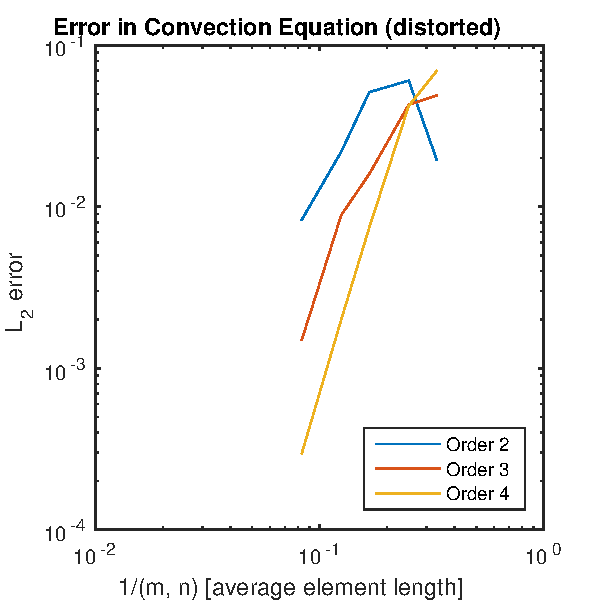
\includegraphics[scale=0.8]{cc_err_distort.pdf}
\end{tabular}
\caption{$L_2$ error for both the regular (left) and distorted (right) meshes. The second order elements converge as expected, but the higher order elements seem to be slightly underperforming. I am not sure if this is due to the temporal error. Rates are given in table \ref{tbl:cc}. The distortion does not seem to affect the rate much.}
\label{fig:cc}
\end{figure}

\begin{table}[!ht]
\centering
\caption{Table of convergence rates for regular and distorted elements.}
\label{tbl:cc}
\begin{tabular}{c c c}
Order & Regular & Distorted \\
\midrule
2 & 2.98247 & 2.61016\\
3 & 3.51268 & 3.47745 \\
4 & 4.38533 & 4.64987 \\
\end{tabular}
\end{table}

\section{rinvexpl.m Implementation}
Please see the code located at \texttt{2DG.3/dgker/myrinvexpl.m} in the zip file accompanying this report.

\section{Wave Equation}
From inspection, we see that if we have a grid with odd number of subdivisions n, the (n+1)/2 innermost concentric grid line goes through (e, 0).

\section{Euler Equations}

\end{document}
